\documentclass[
aip,
jcp,
%preprint,
reprint,
]{revtex4-1}
%
\usepackage[hyperindex,breaklinks,hidelinks,colorlinks,citecolor=blue]{hyperref}
\usepackage{amsmath, amsthm, amssymb}    
\usepackage{float}
%
\usepackage{graphicx}
\DeclareGraphicsExtensions{.pdf,.eps,.png}
\graphicspath{{Figures/}}
\usepackage[outdir=Figures/]{epstopdf}
\newcommand{\figscale}{0.8}
%
\usepackage{natmove}
%
%\usepackage{mathtools}
%\mathtoolsset{showonlyrefs}
%
\DeclareMathOperator\arctanh{arctanh}
\DeclareMathOperator\arcsinh{arcsinh}
\DeclareMathOperator\sech{sech}
%
\newcommand{\mt}[1]{\boldsymbol{\mathbf{#1}}}          % matrix symbol
\newcommand{\vt}[1]{\boldsymbol{\mathbf{#1}}}          % vector symbol
\newcommand{\tr}[1]{#1^\text{t}}                       % transposition
\newcommand{\diff}[2]{\frac{\partial #2}{\partial #1}} % derivative
\newcommand{\avg}[1]{\overline{#1}}                    % average
\newcommand{\Liu}{\mathcal{L}}
\newcommand{\Ham}[1]{{\mathcal H}_\mathrm{#1}}         % Hamiltonian
%\newcommand{\grad}[2]{\nabla_{#1}{#2}}                 % gradient
\newcommand{\grad}[2]{\diff{#1}{#2}}                   % gradient

% Symbols:
\newcommand{\nn}{n}

% Temporary:
\usepackage{soul}

\begin{document}

\author{Charlles R. A. Abreu}
\email{abreu@eq.ufrj.br}
\affiliation{Chemical Engineering Department, Escola de Qu\'imica, Universidade Federal do Rio de Janeiro, Rio de Janeiro, RJ 21941-909, Brazil}
\affiliation{Department of Chemistry, New York University, New York, New York 10003, USA}

\author{Mark E. Tuckerman}
\email{marktuckerman@nyu.edu}
\affiliation{Department of Chemistry, New York University, New York, New York 10003, USA}
\affiliation{Courant Institute of Mathematical Sciences, New York University, New York, New York 10012, USA}
\affiliation{NYU-ECNU Center for Computational Chemistry at NYU Shanghai, Shanghai 200062, China}

\title{New Methods for Multiple Time-Scale Molecular Dynamics with Very Large Time Steps}

\keywords{molecular dynamics; multiple time-stepping; resonance}

\date{\today}

\maketitle

\section{Introduction}

Multiple time-scale (MTS) integration \cite{Grubmuller_1991, Tuckerman_1992, Martyna_1996} is an effective way of improving the efficiency of Molecular Dynamics (MD) simulations.
In classical MD, it allows the most expensive computations, such as the evaluation of long-range van der Waals and electrostatic components of a force field, to be done less frequently than others.
This is possible because the time scale of variations in such contributions is much larger than those in both non-bonded interactions at short distances and bonded intramolecular forces.
If estimating ensemble averages is the main goal of a simulation, then the maximum benefit one can get from multiple time-stepping occurs when it is possible to match the longest-scale step size with the correlation time of the system dynamics, i.e., the sampling period required to obtain a series of uncorrelated configurations.
Although this is theoretically feasible in many situations, it took long until the capacity of the MTS strategy could be fully realized in them.
The cause of this delay is the existence of resonance artifacts \cite{Biesiadecki_1993, Schlick_1998a, Ma_2003} that constrain the maximum attainable step size.
Attempts have been made over the years to overcome this limitation.
One of the strategies, known as mollified impulse \cite{Garcia-archilla_1998, Skeel_1999}, relies on altering the slow part of the potential energy function.
This is done by evaluating the corresponding forces at filtered positions, averaged along auxiliary trajectories which are, in turn, dictated by the fast part of the potential.

The most successful approach for dealing with resonance artifacts in thermostatted MD does not involve altering the potential.
Instead, it entails introducing new dynamic variables (extended system approach) and enforcing isokinetic constraints \cite{Minary_2003a, Minary_2003b, Minary_2004, Leimkuhler_2013}.
The basic recipe consists in pairing an extra velocity with the actual velocity of each degree of freedom in the system.
Then, independent thermostats are attached to all extra velocities.
However, instead of letting them vary without limits, the combined kinetic energy of each velocity pair is enforced to be constant.
In this way, the magnitude of every actual velocity can never exceed a certain value, thus avoiding resonance and instability in the simulated dynamics.
This procedure is clearly not meant to reproduce the Maxwell-Boltzmann distribution of velocities of a canonical ensemble, but it provably provides the correct distribution of coordinates \cite{Minary_2003a, Minary_2003b, Minary_2004, Leimkuhler_2013}.
In a more elaborate version, several extra velocities (with their attached thermostats) are associated to each degree of freedom and take part in the isokinetic constraints.
The method was originally formulated \cite{Minary_2003a, Minary_2003b, Minary_2004} with deterministic thermostats \cite{Martyna_1992} and subsequently reformulated \cite{Leimkuhler_2013} with stochastic ones \cite{Samoletov_2007, Leimkuhler_2009}.

There is a rich literature on the development and analysis of extended-system methods \cite{Martyna_1996, Tuckerman_1999, Tuckerman_2001a, Sergi_2001, Ezra_2004, Tuckerman_2010}.
Pioneered in the 1980's \cite{Andersen_1980, Nose_1984, Hoover_1985}, they allowed the use of MD to study thermodynamic systems under the influence of external baths.
Nevertheless, the isokinetic formulation is somewhat extraneous in such universe.
Some of the well-established tools developed in the area are not readily applicable to its analysis.
As a consequence, knowledge about the properties of isokinetic methods has been advancing in a case-by-case basis.
Once this is the first approach that allows MTS simulations with very large time steps, it becomes particularly hard to distinguish the actual cause of observed anomalies.

In the present paper, we introduce a novel resonance-control methodology and demonstrate that it is completely equivalent to the isokinetic framework.
It consists in substituting the kinetic part of the system Hamiltonian by a new momentum-dependent function, whose main feature is also causing the confinement of velocities to a fixed range.
The potential part of the Hamiltonian is kept unchanged.
We are, thus, recasting the isokinetic approach is a form that is more akin to standard extended-system and stochastic methods.
This allowed us to unveil certain properties of the isokinetic dynamics which remained hitherto unnoticed, such as 1) the driven-variable nature of the extra velocities, 2) the existence of additional conserved quantities, and 3) some odd forms of velocity frequency distributions.
More importantly, it became straightforward to devise a new, Langevin-type version of the method with superior performance.

\section{Methods}
\label{sec:methods}

\subsection{Molecular Dynamics in the Canonical Ensemble}
\label{sec:standard canonical ensemble}

For a classical system with coordinates represented by $\vt r$, we are often interested in obtaining canonical-ensemble averages of a purely configurational property, say,
\begin{equation*}
\label{eq:configurational average}
\langle A \rangle = \frac{1}{Z} \int e^{-\frac{U(\vt r)}{kT}} A(\vt r) d\vt r,
\end{equation*}
where $T$ is the temperature, $k$ is the Boltzmann constant, $U(\vt r)$ is a potential energy function, and $Z$ is a normalizing constant.
This is usually accomplished by defining a standard Hamiltonian $\mathcal{H}(\vt r, \vt p) = U(\vt r) + \sum_{i=1}^{N_f} \frac{p_i^2}{2 m_i}$ and exploring the phase space by means of some canonical (constant NVT) dynamics method.
In this expression, $p_i$ is the conjugate momentum and $m_i$ is the mass associated to a degree of freedom $i$, whose total number is $N_f$.
This procedure results in a probability density $\rho(\vt r, \vt p) \propto e^{-\frac{\mathcal{H}(\vt r, \vt p)}{kT}}$, up to small systematic deviations introduced by the numerical discretization of time \cite{Eastwood_2010, Davidchack_2010, Silveira_2017a, Silveira_2019a}.
As a result, coordinates are sampled with the desired probabilities and, at the same time, each momentum $p_i$ fluctuates according to a zero-mean, normal distribution with standard deviation $\sigma_i = \sqrt{m_i k T}$.

In a Hamiltonian dynamics, as well as in most non-Hamiltonian methods devised to sample the canonical ensemble, the velocity of a particle is the gradient of $\mathcal{H}$ with respect to its momentum, that is,
\begin{equation}
\label{eq:velocity as momentum gradient}
v_i = \diff{p_i}{{\mathcal H}}.
\end{equation}

Therefore, in a simulation with the standard Hamiltonian, in which $v_i = \frac{p_i}{m_i}$, a large displacement will take place whenever the absolute value of some momentum increases excessively due to the action of a large force.
Time discretization can cause such forces to emerge due to, for instance, spurious atomic overlaps, thus causing numerical instability.
Massive isokinetic methods \cite{Minary_2003a, Minary_2003b, Minary_2004, Leimkuhler_2013} manage to avoid this problem by setting an upper bound to the kinetic energy of every degree of freedom.
Therefore, the largest single-step displacement that a coordinate $r_i$ can undergo during a massive isokinetic simulation is $c_i \delta t$, where $\delta t$ is the size of each time step (or inner time step, in the case of a multiple time-scale simulation) and $c_i$ is the speed limit imposed to such degree of freedom.
A side-effect of this strategy is that the probability distribution of velocities is no longer Gaussian, as it is in a standard canonical ensemble, but has a particular form that depends on the number of thermostats attached to each degree of freedom \cite{Abreu_2020}.
On one hand, the details of the velocity and momentum distributions are not particularly relevant if one is only interested in configurational averages.
On the other hand, the mixing time can actually be affected, thus altering the efficiency with which the coordinate space is sampled.
We have shown \cite{Abreu_2020} that, on average, each atom is slower in an isokinetic dynamics than it would be in a standard dynamics at the same temperature.

\subsection{New Hamiltonian for Regulated Isothermal Dynamics}
\label{sec:new hamiltonian}

Inspired by the massive isokinetic methods \cite{Minary_2003a, Minary_2003b, Minary_2004, Leimkuhler_2013}, we propose a new approach to impose a speed limit $c_i$ to every degree of freedom of a dynamical system.
This approach, which we will refer to as \textit{regulated dynamics}, consists in using a modified Hamiltonian, given by
\begin{equation}
\label{eq:modified hamiltonian}
\mathcal{H}_\nn(\vt r, \vt p) = U(\vt r) + \nn kT \sum_{i=1}^{N_f} \ln \cosh\left(\sqrt{\frac{\alpha_\nn}{\nn m_i k T}} p_i\right),
\end{equation}
where $\nn > 0$ is an arbitrary parameter and $\alpha_\nn$ is a function of $\nn$, whose form is to be determined so that $\mathcal{H}_\nn$ meets some desirable features.

The new Hamiltonian shares important properties with the standard one.
For instance, by being an even function of every $p_i$, it is invariant to momentum sign flips.
Moreover, it is separable with respect to the set of coordinates and to every individual momentum, which makes the marginal equilibrium distributions of $\vt r$ and $\vt p$ independent of each other, as well as those of $p_i$ and $p_j$ whenever $i \neq j$.
Together with the condition that $e^{-\frac{\mathcal{H}_\nn(\vt r, \vt p)}{k T}} \to 0$ when any $p_i \to \pm \infty$, such separability renders valid  \cite{Uline_2008} the generalized equipartition theorem \cite{Tolman_1918a}, which states that
\begin{equation}
\label{eq:generalized equipartition}
\left\langle v_i p_i \right\rangle = k T.
\end{equation}

One desirable feature of $\mathcal{H}_\nn$ is that it approaches the standard Hamiltonian when $\nn$ increases.
By observing the Taylor series expansion
\begin{equation*}
\nn \ln \cosh\left(\sqrt{\frac{\alpha_\nn}{\nn}} x\right) = \frac{\alpha_\nn x^2}{2} - \frac{\alpha_\nn^2 x^4}{12 \nn} + \frac{\alpha_\nn^3 x^6}{45 \nn^2} + \mathcal{O}(x^8),
\end{equation*}
it becomes clear that this function will converge to $\frac{1}{2}x^2$ if $\alpha_\nn$ fulfills the limiting condition
\begin{equation}
\label{eq:alpha convergence condition}
\lim\limits_{\nn \to \infty} \alpha_\nn = 1,
\end{equation}
thus making $\mathcal{H}_\infty = \mathcal{H}$.
If a constant-NVT simulation is set up with the new Hamiltonian, coordinates will still be sampled proportionally to $e^{-\frac{U(\vt r)}{kT}}$, as it was designed to do, while each momentum $p_i$ will be sampled according to a probability density given by
\begin{equation}
\label{eq:momentum distribution}
\rho_\nn(p_i) = \sqrt{\frac{\alpha_\nn}{\nn m_i k T}} \frac{\Gamma\left(\frac{\nn+1}{2}\right)}{\Gamma\left(\frac{\nn}{2}\right) \sqrt{\pi}} \sech^\nn\left(\sqrt{\frac{\alpha_\nn}{\nn m_i k T}} p_i\right),
\end{equation}
where $\Gamma$ is the complete gamma function.
This probability density, whose normalization constant is obtained in Appendix \ref{sec:momentum and velocity distributions}, is depicted in the top row of Fig.~\ref{fig:momentum and velocity functions} for two instances of $\alpha_\nn$ satisfying Eq.~\eqref{eq:alpha convergence condition} and for various integer values of $\nn$.
The tendency towards the normal distribution with increasing $\nn$ is evident.
The figure also depicts, in its middle row, the relation between velocity and momentum for the same combinations of $\alpha_\nn$ and $\nn$.
Such relation, obtained from Eqs.~\eqref{eq:velocity as momentum gradient} and \eqref{eq:modified hamiltonian}, is
\begin{equation}
	\label{eq:velocity definition}
	v_i = c_i \tanh\left(\frac{\alpha_\nn p_i}{m_i c_i}\right),
\end{equation}
	where the speed limit $c_i$ is given by
\begin{equation}
	\label{eq:speed limit definition}
	c_i = \sqrt{\frac{\alpha_\nn \nn k T}{m_i}}.
\end{equation}

\begin{figure}[htbp!]
	\centering
	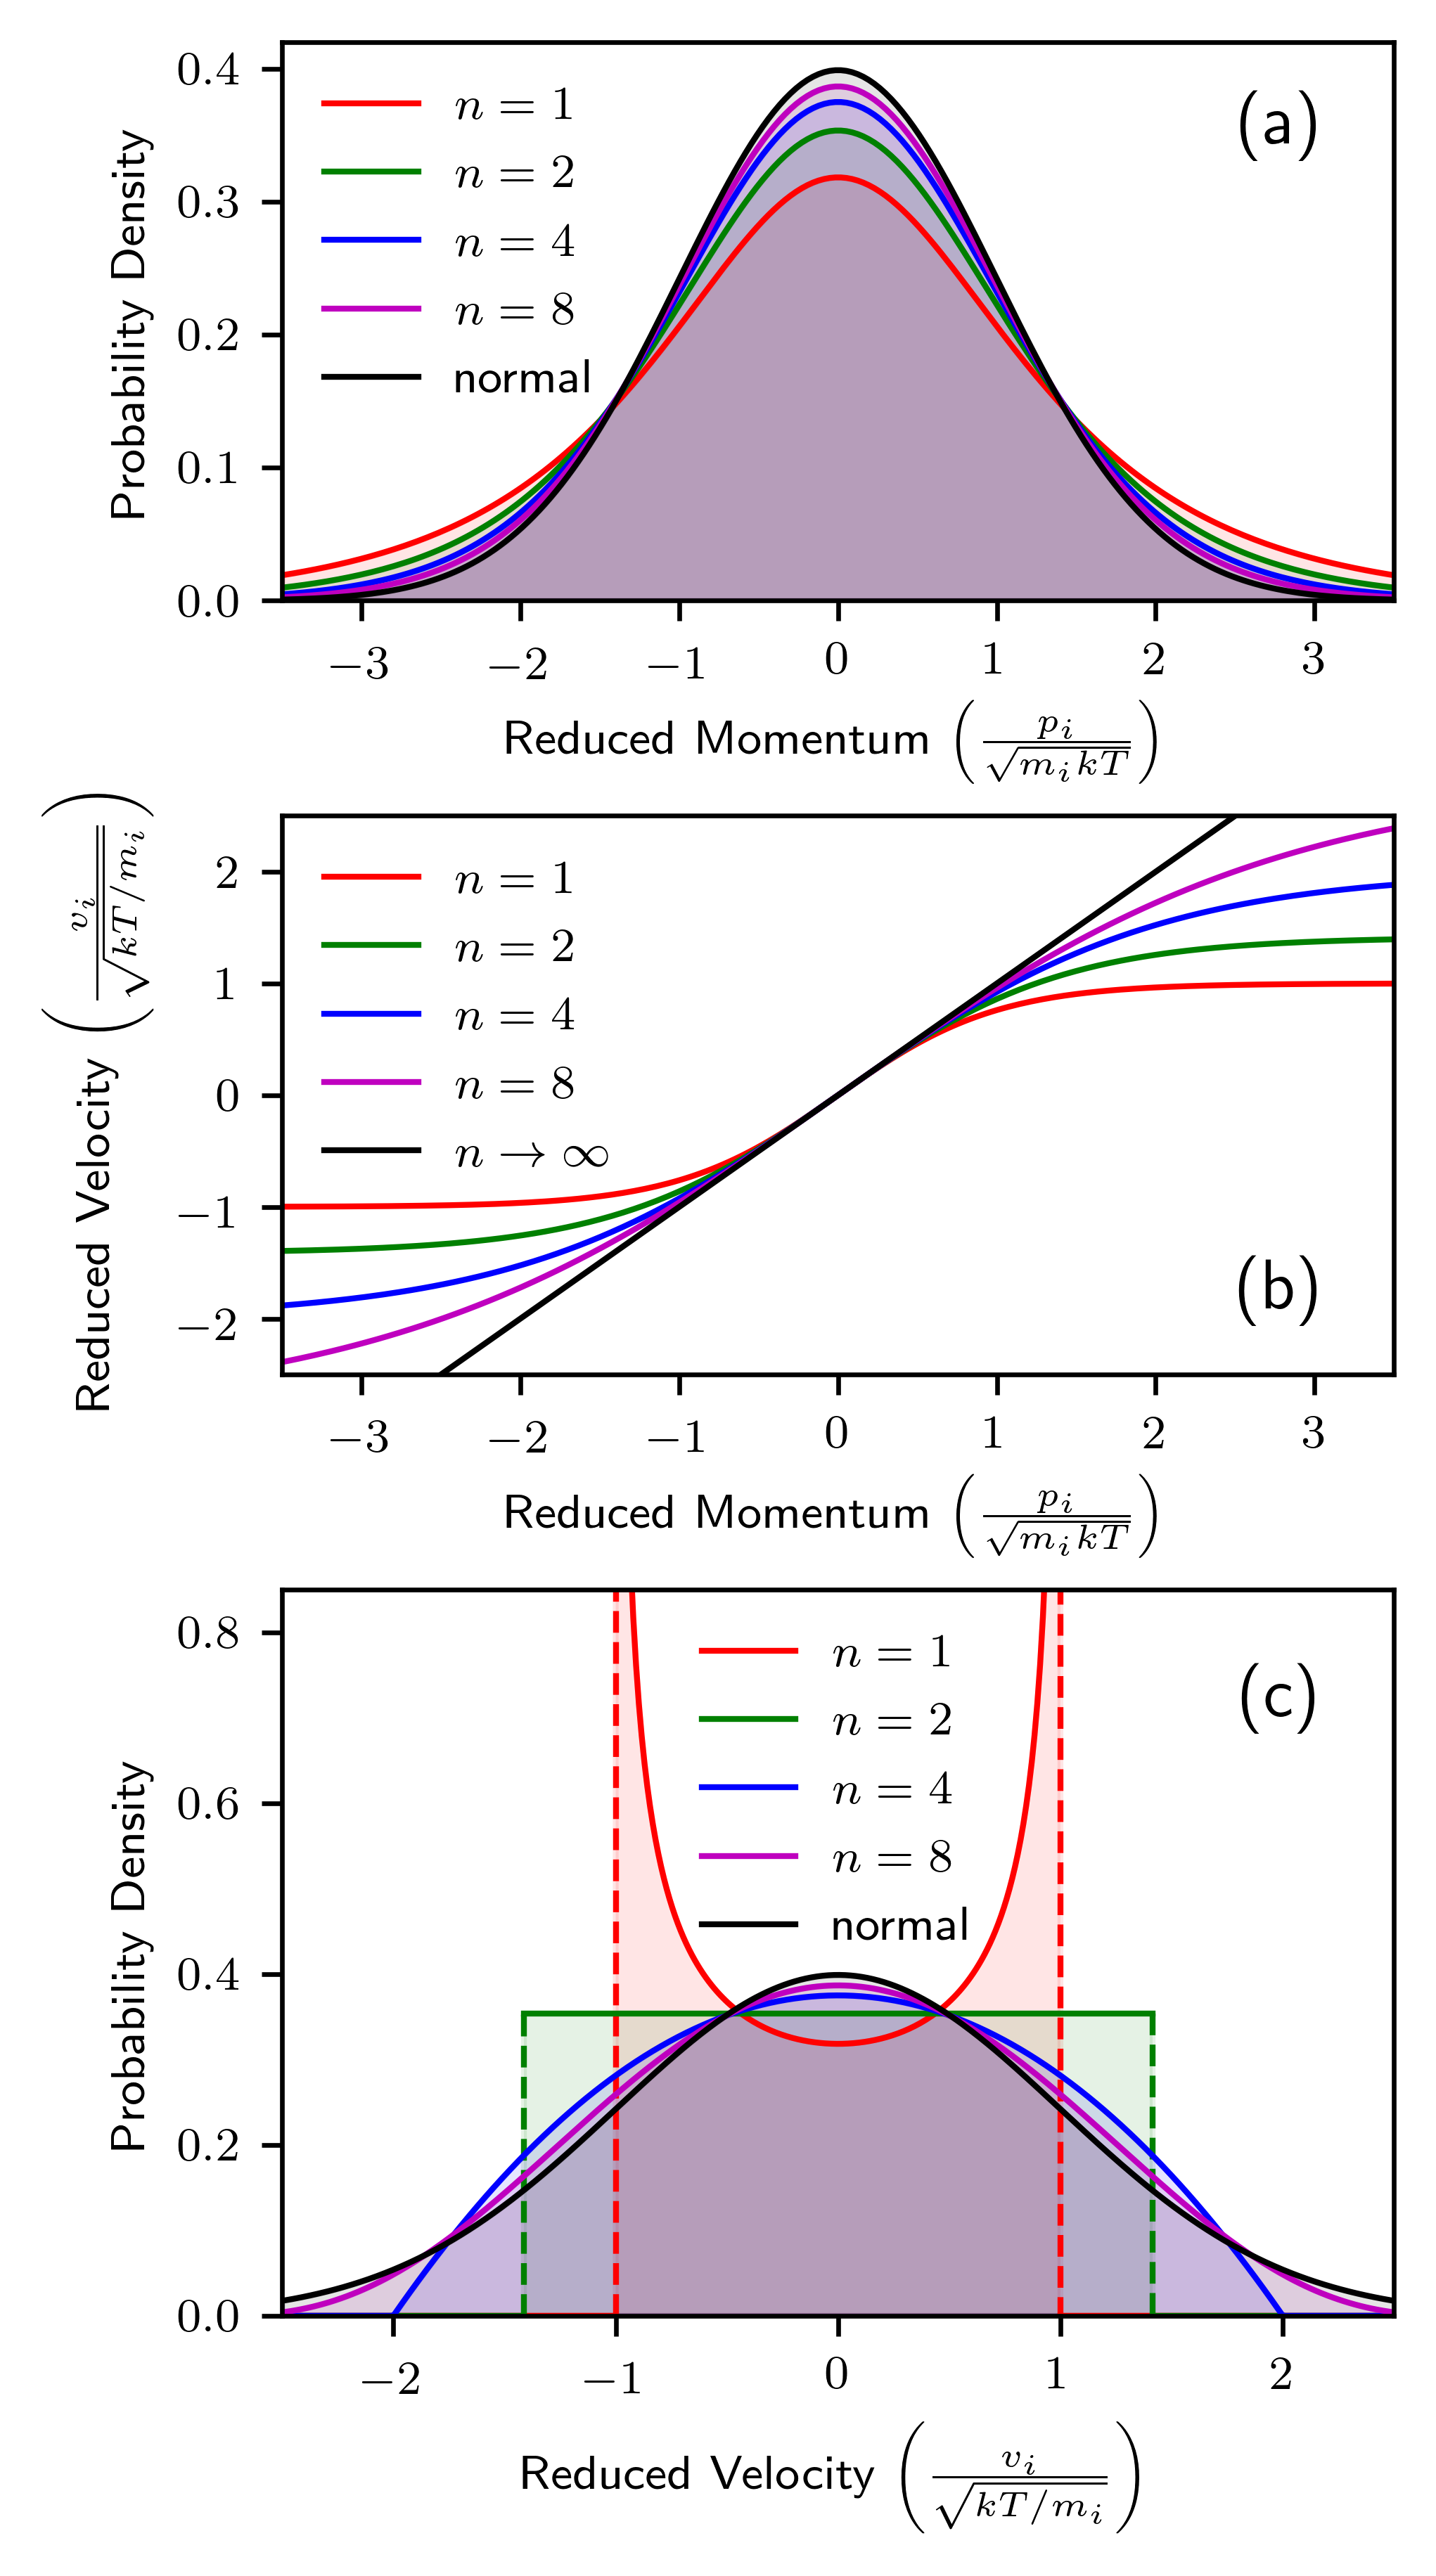
\includegraphics[width=\linewidth]{momentum_and_velocity_functions}
	\caption{Momentum distributions (top) and velocities (bottom)}
	\label{fig:momentum and velocity functions}
\end{figure}

It is interesting to observe the distribution of velocities, whose PDF is derived in Appendix \ref{sec:momentum and velocity distributions} and is given by
\begin{equation*}
\varrho_\nn(v_i) = \begin{cases}
\frac{1}{c_i} \frac{\Gamma\left(\frac{\nn+1}{2}\right)}{\Gamma\left(\frac{\nn}{2}\right) \sqrt{\pi}} \left(1-\frac{v_i^2}{c_i^2}\right)^{\frac{\nn}{2}-1} & \mathrm{if} \; v_i^2 \leq c_i^2 \\
0 & \mathrm{otherwise}
\end{cases}.
\end{equation*}

This distribution is depicted in the bottom row of Fig.~\ref{fig:momentum and velocity functions} for the same choices of $\alpha_\nn$ and $\nn$ employed before.
If $\alpha_\nn = 1$ and $\nn \in \mathbb{N}$, it becomes identical to the distribution corresponding to the massive isokinetic dynamics \cite{Abreu_2020}, with parameter $\nn$ substituting the number $L$ of thermostats attached to each degree of freedom.
One important aspect of this distribution, which will be essential in the forthcoming discussion about thermostat algorithms, is its implied special form of the kinetic energy equipartition (see Appendix~\ref{sec:momentum and velocity distributions}), given by
\begin{equation}
\label{eq:special kinetic energy equipartition}
\left\langle m_i v_i^2 \right\rangle = \frac{\alpha_\nn \nn}{\nn+1} kT.
\end{equation}

There is only one form for the function $\alpha_\nn$ that renders the relation above always equivalent to the kinetic energy equipartition of the standard canonical ensemble, which is $\alpha_\nn = \frac{\nn+1}{\nn}$.
Otherwise, the equivalency is approached only if $\nn$ is large.
If $\alpha_\nn = 1$, it is approached from below, meaning that particles are slower, on average, than their counterparts in a canonical ensemble at the same temperature.
This has been observed in the case of massive isokinetic dynamics methods \cite{Abreu_2020}, with implications in their capability of producing uncorrelated samples for configurational property inference.
With a single thermostat per degree of freedom ($L=1$), for instance, the mean kinetic energy of the system is only half the value corresponding to a standard canonical ensemble.
On the other hand, $\alpha_\nn = 1$ is the only option that makes, regardless of the value of parameter $\nn$, $v_i \to \frac{p_i}{m_i}$ when $p_i$ is small.
This can be observed in the middle row of Fig.~\ref{fig:momentum and velocity functions}, with all curves collapsing to the diagonal line around $p_i = 0$ when $\alpha_\nn = 1$.
As a consequence, the peak of the momentum distribution has a similar shape for all $\nn$, with marked differences occurring only in the tail regions.
Therefore, each particle will most likely move in approximately the same direction of its momentum vector, which is in turn guided by the forces acting upon it, thus resembling the dynamics (not only the equilibrium distribution) of a canonical ensemble.
In Sec.~\ref{}, we will test the implications of choosing either $\alpha_\nn = 1$ or $\alpha_\nn = \frac{\nn+1}{\nn}$.

In the forthcoming sections, we deal with simulation methods that aim at reproducing a canonical distribution with the new Hamiltonian.
First, we employ a massive version of an existing thermostat algorithm and show that it simply relies on the validity of the generalized equipartition theorem, Eq.~\eqref{eq:generalized equipartition}, in order to enact correct thermostatting.
Next, we devise a new algorithm which, instead, relies on the especial equipartition given by Eq.~\eqref{eq:special kinetic energy equipartition}.
A marked difference between these two fundamental equations is that the quantity subject to equipartition in the former is unbounded, as $p_i$ is, while its counterpart in the latter has an upper bound in $m_i c_i^2$.
Finally, it is worth mentioning that it would also be possible to use higher-order central moments (see Appendix~\ref{sec:momentum and velocity distributions}) for enacting thermostatting, such as in the Generalized Gaussian Moment algorithm \cite{Liu_2000}, but this is beyond the scope of this article.

\subsection{Regulated Nos\'{e}-Hoover-Langevin Thermostatting}
\label{sec:regulated massive NHL thermostatting}

In order to derive equations of motion for a regulated NVT dynamics in the space of coordinates $\vt r$ and momenta $\vt p$, referred to hereafter as the physical phase space, we employ a massive version of the Nos\'{e}-Hoover-Langevin (NHL) method \cite{Samoletov_2007, Leimkuhler_2009}.
This begins by extending the phase space with $N_f$ extra pairs of coordinates $\vt \eta$ and conjugate momenta $\vt p_\eta$.
An inertial parameter $Q = kT \tau^2$ is associated to every degree of freedom, with $\tau$ being a characteristic time scale.
The dynamics of the NHL method is described by a system of stochastic differential equations (SDE) expressed as
\begin{subequations}
	\label{eq:regulated massive NHL equations}
	\begin{align}
	&dr_i = v_i dt, \\
	&dp_i = (F_i - v_{\eta_i} p_i) dt, \quad \mathrm{and} \\
	&dp_{\eta_i} = (p_i v_i - kT) dt - \gamma p_{\eta_i} dt + \sqrt{2 \gamma Q kT} dW_i,
	\end{align}
\end{subequations}
where $F_i = -\diff{r_i}{U}$ is the force exerted on $i$,
$v_{\eta_i} = \frac{p_{\eta_i}}{Q}$ is the rate of change of $\eta_i$,
$\gamma$ is a friction constant, and
$dW_i$ denotes an infinitesimal increment of a Wiener process.
Each velocity $v_i$ is computed via Eq.~\eqref{eq:velocity definition}, which is the single difference between the regulated and standard versions of the massive NHL method.
It is worth noting that an equation $d\eta_i = v_{\eta_i} dt$ for each $i$ could have also been included, but they can be ignored in practice for having no influence on the physical-space dynamics.
Nevertheless, it is important from a theoretical standpoint when it comes to demonstrating that such space is correctly sampled in accordance with $e^{-\frac{\mathcal{H}_\nn(\vt r, \vt p)}{kT}}$.

Although the main advantage of the proposed method takes place in the context of multiple time-scale simulations, we begin by presenting a single time-scale integration scheme, which can be easily extended afterwards.
As it has been demonstrated in recent years \cite{Leimkuhler_2013b, Zhang_2017, Li_2017, Fass_2018, Zhang_2019}, middle-type integration schemes are very accurate at reproducing the distribution of coordinates, at the expense of the distribution of velocities.
This is particularly appealing for the present method, given its pursued characteristics.
In the usual operator splitting notation, the time steps of our proposed middle-scheme integrator is \cite{Zhang_2017}
\begin{equation*}
e^{\delta t\Liu} = e^{\frac{\delta t}{2} \Liu^\mathrm{T}_p} e^{\frac{\delta t}{2} \Liu^\mathrm{T}_r} e^{\delta t\Liu_\mathrm{bath}} e^{\frac{\delta t}{2} \Liu^\mathrm{T}_r} e^{\frac{\delta t}{2} \Liu^\mathrm{T}_p},
\end{equation*}
where
\begin{equation*}
e^{\delta t\Liu_\mathrm{bath}} = e^{\frac{\delta t}{2} \Liu^\mathrm{T}_{v_\eta}} e^{\frac{\delta t}{2} \Liu^\mathrm{S}_p} e^{\delta t \Liu^\mathrm{O}_{v_\eta}} e^{\frac{\delta t}{2} \Liu^\mathrm{S}_p} e^{\frac{\delta t}{2} \Liu^\mathrm{T}_{v_\eta}}.
\end{equation*}

In the propagators above, a superscript index $\mathrm{T}$ stands for translation, meaning that the effects of propagators $e^{t \Liu^\mathrm{T}_r}$, $e^{t \Liu^\mathrm{T}_p}$, and $e^{t \Liu^\mathrm{T}_{v_\eta}}$ on each degree of freedom $i$ can be expressed, respectively, as
\begin{align}
&r_i = r_i^0 + v_i^0 t, \label{eq:NHL move}\\
&p_i = p_i^0 + F_i^0 t, \quad \mathrm{and} \\
&v_{\eta_i} = v_{\eta_i}^0 + \frac{p_i^0 v_i^0 - kT}{Q} t,
\end{align}
where a superscript $0$ denotes the initial condition encountered by the propagator and $t$ corresponds to the time span of its action.
In turn, superscript $\mathrm{S}$ means scaling, so that $e^{t \Liu^\mathrm{S}_p}$ is a propagator whose action on each momentum $p_i$ is
\begin{equation}
p_i = p_i^0 e^{-v_{\eta_i}^0 t}.
\end{equation}

Finally, superscript $\mathrm{O}$ refers to an Ornstein-Uhlenbeck stochastic process, so that the action of $e^{t \Liu^\mathrm{O}_{v_\eta}}$ on each thermostat variable $v_{\eta_i}$ can be executed as
\begin{equation}
v_{\eta_i} = v_{\eta_i}^0 e^{-\gamma t} + \sqrt{\tfrac{kT}{Q}(1 - e^{-2\gamma t})} \xi_i,
\end{equation}
where $\xi_i$ is an independent random variate following the standard normal probability distribution.
%Notice that, as explained before, we did not need to include integration steps for $\vt \eta$.
Implementing the described propagators might be straightforward once a computer code is available for evaluating the forces at every time step.

We now demonstrate that the Boltzmann-Gibbs distribution of coordinates is correctly obtained.
As in Ref.~\citenum{Leimkuhler_2013}, we do it in two steps.
First, we derive the equilibrium distribution of the method in its deterministic form, that is, with $\gamma=0$.
Then, we show that the stochastic contribution keeps such distribution invariant.
The deterministic version of Eq.~\eqref{eq:regulated massive NHL equations} is a massive Nos\'e-Hoover \cite{Nose_1984, Hoover_1985} thermostat applied to $\mathcal{H}_\nn$ as expressed in Eq.~\eqref{eq:modified hamiltonian}.
It is a non-Hamiltonian dynamics that conserves an energy function defined as
\begin{equation}
\label{eq:extended energy}
H_\nn(\vt r, \vt p, \vt \eta, \vt p_\eta) = {\mathcal H}_\nn(\vt r, \vt p) + \sum_{i=1}^{N_f} \left(k T \eta_i + \frac{p_{\eta_i}^2}{2 Q} \right).
\end{equation}

A set of equations of motion devised to preserve $H_\nn$ can be written in the general form \cite{Sergi_2001}
\begin{equation}
\label{eq:general conservative phase-space flow}
\dot{\vt x} = {\mt B} \grad{\vt x}{H_\nn},
\end{equation}
where $\vt x$ is the vector of all extended phase-space variables, $\mt B$ is a skew-symmetric, matrix-valued function of $\vt x$, and $\grad{\vt x}{}$ is the gradient operator.
By virtue of the chain rule, the time derivative of any scalar function $f(\vt x)$ is given by $\dot f = \tr{\dot{\vt x}}\grad{\vt x}{f} = \tr{(\grad{\vt x}{H_\nn})} \tr{\mt B} (\grad{\vt x}{f})$.
This is a quadratic form, which becomes identically null whenever its defining matrix is skew-symmetric.
Hence, $\dot{H}_\nn = 0$.
For a massive thermostatting approach, both $\mt B$ and $\grad{\vt x}{H_\nn}$ can be organized blockwisely, with $\mt B$ having a block-diagonal structure.
In the case of a Nos\'e-Hoover dynamics, the blocks defined for each degree of freedom $i$ will be
\begin{equation}
\label{eq:regulated dynamics diagonal block}
{\mt B}_{i,i} =
\left[\begin{array}{cccc}
	0  &  1  & 0  &  0   \\
	-1 &  0  & 0  & -p_i \\
	0  &  0  & 0  &  1   \\
	0  & p_i & -1 &  0
\end{array}\right]
\quad \mathrm{and} \quad
\grad{\vt x_i}{H_\nn} =
\left[\begin{array}{c}
	   -F_i    \\
	   v_i     \\
	   k T     \\
	v_{\eta,i}
\end{array}\right].
\end{equation}

Note that the entries of $\grad{\vt x_i}{H_\nn}$ are the derivatives of ${H_\nn}$ with respect to $r_i$, $p_i$, $\eta_i$, and $p_{\eta_i}$, respectively.
All this development will prove useful once again in Sec.~\ref{sec:twice-regulated massive NHL thermostatting}, where we derive a different method which also preserves $H_\nn$.
Now, it follows from Eqs.~\eqref{eq:general conservative phase-space flow} and \eqref{eq:regulated dynamics diagonal block} that
\begin{subequations}
	\label{eq:massive Nose-Hoover equations}
	\begin{align}
	&\dot{r}_i = v_i, \\
	&\dot{p}_i = F_i - v_{\eta_i} p_i, \\
	&\dot{\eta}_i = v_{\eta_i}, \quad \mathrm{and} \\
	&\dot{p}_{\eta_i} = v_i p_i - kT, \label{eq:massive Nose-Hoover p_eta}
	\end{align}
\end{subequations}
which is an ODE system that matches Eqs.~\eqref{eq:regulated massive NHL equations} in the deterministic limit.
By contrasting Eq.~\eqref{eq:massive Nose-Hoover p_eta} to Eq.~\eqref{eq:generalized equipartition}, we realize that described method has its base on the generalized equipartition theorem.

In order to apply the phase-space analysis method developed in Refs.~\citenum{Tuckerman_1999} and \citenum{Tuckerman_2001a}, we need to determine the phase space compressibility, which is defined as
\begin{equation}
\label{eq:phase space compressibility}
\kappa = \nabla_{\vt x} \cdot \dot{\vt x}.
\end{equation}

In the case of Eq.~\eqref{eq:massive Nose-Hoover equations}, the compressibility is
\begin{equation}
\label{eq:Nose-Hoover compressibility}
\kappa = -\sum_{i=1}^{N_f} v_{\eta_i} = -\dot{\eta}_\mathrm{sum}.
\end{equation}
where $\dot{\eta}_\mathrm{sum} = \sum_{i=1}^{N_f} \eta_i$.
A flow like Eq.~\eqref{eq:general conservative phase-space flow} takes place in a manifold $H_\nn(\vt x) = H_\nn^0$, where $H_\nn^0$ is a constant that depends on the initial condition.
If this dynamics is ergodic and $H_\nn$ is the only conserved quantity, then the partition function of the resulting ensemble can be expressed as \cite{Tuckerman_1999, Tuckerman_2001a}
\begin{equation}
\label{eq:partition function definition}
\Omega = C \int \delta\Big(H_\nn(\vt x) - H_\nn^0\Big) \sqrt{g} d{\vt x},
\end{equation}
where $\delta(\cdot)$ is the Dirac delta function,
$\sqrt{g}$ is a metric determinant, and
$C$ is the proper statistical-mechanical prefactor, whose form is irrelevant for the present analysis.
For a system with internal forces only, Eq.~\eqref{eq:massive Nose-Hoover equations} also preserves quantities related to the sum of all momenta at each spatial dimension.
However, we can ignore these conservation laws here as we will eventually include a stochastic component to the equations of motion.
This way, according to Refs.~\citenum{Tuckerman_1999} and \citenum{Tuckerman_2001a}, we must simply substitute $e^{-w}$ for $\sqrt{g}$ in Eq.~\eqref{eq:partition function definition}, where $w$ is defined so that $\dot{w} = \kappa$ \cite{Tuckerman_1999, Tuckerman_2001a}.
Therefore, it follows from Eq.~\eqref{eq:Nose-Hoover compressibility} that
\begin{multline}
\label{eq:partition function result}
\Omega = C \int \delta\Big(H_\nn(\vt x) - H_\nn^0\Big) e^{\eta_\mathrm{sum}} d{\vt x} = \\
= \frac{C e^{-\frac{H_\nn^0}{kT}}}{kT} \int e^{-\frac{\mathcal{H}_\nn(\vt r, \vt p) + \frac{1}{2 Q} \|{\vt p}_\eta\|^2}{kT}} d{\vt r} d{\vt p} d{\vt p}_\eta,
\end{multline}
where integration has been carried out for all $\eta_i$ after replacing $H_\nn(\vt x)$ from Eq.~\eqref{eq:extended energy}.
This result clearly shows that the marginal distribution in the physical phase space will be proportional to $e^{-\frac{\mathcal{H}_\nn(\vt r, \vt p)}{kT}}$.

\hl{Show that Langevin operator does not change the distribution}

\subsection{Regulated Thermostatting Based on the Special Kinetic Energy Equipartition}
\label{sec:twice-regulated massive NHL thermostatting}

We now propose a different version of the massive NHL algorithm, whose thermostatting capability relies on the special form of the kinetic energy equipartition expressed in Eq.~\eqref{eq:special kinetic energy equipartition}.
Based on the developments of Sec.~\ref{sec:regulated massive NHL thermostatting}, we begin by describing the deterministic version of the method before including a Langevin-type thermostat.
The new equations of motion can be obtained by simply modifying some entries of the matrix $\mt B$, which is present in Eqs.~\eqref{eq:general conservative phase-space flow} and \eqref{eq:regulated dynamics diagonal block}, while maintaining its skew-symmetric and block-diagonal structures.
Each block in the main diagonal of the modified matrix is
\begin{equation}
{\mt B}_{i,i} =
\left[
\begin{array}{cccc}
	0  &             1              &            0             &              0              \\
	-1 &             0              &            0             & -\frac{m_i v_i}{\alpha_\nn} \\
	0  &             0              &            0             &   1 - \frac{v_i^2}{c_i^2}   \\
	0  & \frac{m_i v_i}{\alpha_\nn} & -1 + \frac{v_i^2}{c_i^2} &              0
\end{array}
\right].
\end{equation}

As a result, Eq.~\eqref{eq:general conservative phase-space flow} becomes
\begin{subequations}
	\label{eq:modified massive Nose-Hoover equations}
	\begin{align}
	&\dot{r}_i = v_i, \\
	&\dot{p}_i = F_i - \frac{v_{\eta_i} m_i v_i}{\alpha_\nn},  \label{eq:modified massive Nose-Hoover p} \\
	&\dot{\eta}_i = v_{\eta_i}\left(1 - \frac{v_i^2}{c_i^2}\right), \quad \mathrm{and} \\
	&\dot{p}_{\eta_i} = \frac{\nn+1}{\alpha_\nn \nn} m_i v_i^2 - kT \label{eq:modified massive Nose-Hoover p_eta}.
	\end{align}
\end{subequations}

We should now contrast Eq.~\eqref{eq:modified massive Nose-Hoover p_eta} to Eq.~\eqref{eq:special kinetic energy equipartition}.
Due to the skew symmetry of $\mt B$, it is straightforward to conclude that the equations above preserve the extended energy defined in Eq.~\eqref{eq:extended energy}.
The phase-space compressibility they imply is $\kappa = - \sum_{i=1}^{N_f} \frac{v_{\eta_i} m_i}{\alpha_\nn} \frac{d v_i}{d p_i}$.
From Eq.~\eqref{eq:velocity definition},
\begin{equation}
\label{eq:velocity derivative wrt momentum}
\frac{d v_i}{d p_i} = \frac{\alpha_\nn}{m_i} \left[1 - \tanh^2\left(\frac{\alpha_\nn p_i}{m_i c_i}\right)\right] = \frac{\alpha_\nn}{m_i} \left(1 - \frac{v_i^2}{c_i^2}\right).
\end{equation}

Therefore,
\begin{equation}
\kappa = - \sum_{i=1}^{N_f} v_{\eta_i} \left(1 - \frac{v_i^2}{c_i^2}\right) = -\dot{\eta}_\mathrm{sum}.
\end{equation}

Remarkably, this results guarantees that the modified method will produce the same partition function as that shown in Eq.\eqref{eq:partition function result} and the same limiting distribution in the physical phase space.
We are now ready to include the stochastic contributions to the equations of motion, which then become
\begin{subequations}
	\label{eq:modified massive Nose-Hoover-Langevin equations}
	\begin{align}
	&dr_i = v_i dt, \\
	&dp_i = \left(F_i - \frac{v_{\eta_i} m_i v_i}{\alpha_\nn}\right) dt, \quad \mathrm{and} \\
	&dp_{\eta_i} = \left(\frac{\nn+1}{\alpha_\nn \nn} m_i v_i^2 - kT\right) dt - \gamma p_{\eta_i} dt + \sqrt{2 \gamma Q kT} dW_i \label{eq:modified massive Nose-Hoover-Langevin p_eta}.
	\end{align}
\end{subequations}

Numerical integration can be done very similarly to the 

Thermostat translation propagator:
\begin{equation*}
v_{\eta_i} = v_{\eta_i}^0 + \frac{1}{Q}\left[\frac{\nn+1}{\alpha_\nn \nn} m_i (v_i^0)^2 - kT\right] t.
\end{equation*}

Scaling propagator is the exact solution of
\begin{equation*}
\dot{p}_i = -\frac{v_{\eta_i} m_i v_i}{\alpha_\nn} = -\frac{v_{\eta_i} m_i c_i}{\alpha_\nn} \tanh\left(\frac{\alpha_\nn p_i}{m_i c_i}\right).
\end{equation*}

By performing a change of variables to $y_i = \sinh(\frac{\alpha_\nn p_i}{m_i c_i})$ and employing the identities $\cosh x \tanh x = \sinh x$ and $\cosh x dx = d\sinh x$, the differential equation above becomes $\dot{y}_i = -v_{\eta_i} y_i$, whose solution is the simple scaling $y_i = y_i^0 e^{-v_{\eta_i} t}$.
Therefore, the action of 
\begin{equation}
p_i = \frac{m_i c_i}{\alpha_\nn} \arcsinh\left[\sinh\left(\frac{\alpha_\nn p_i^0}{m_i c_i}\right)e^{-v_{\eta_i}^0 t}\right].
\end{equation}

\subsection{Close Connection to the Stochastic Isokinetic Nos\'e-Hoover Method}
\label{sec:modified NHC thermostatting}

As we mentioned in Sec.~\ref{sec:new hamiltonian}, a special case of our proposed Hamiltonian, namely when $\alpha_\nn = 1$ and $n \in \mathbb{N}$, generates a canonical ensemble whose velocity distribution equals that of an isokinetic ensemble \cite{Abreu_2020} with $\nn$ thermostats per degree of freedom.
This already attests a close relationship between the two methodologies.
In the present section, we go further to demonstrate that our second proposed set of equations of motion, the one based on the special equipartition relation, produces exactly the same dynamics as the SIN(R) method \cite{Leimkuhler_2013} when $\alpha_\nn = 1$ and $\nn = 1$.

Let us begin by considering the deterministic limit of the method.
First, we eliminate $p_i$ from Eq.~\eqref{eq:modified massive Nose-Hoover p} by resorting to its relation with $v_i$.
From Eqs.~\eqref{eq:speed limit definition} and \eqref{eq:velocity derivative wrt momentum}, we can obtain that
\begin{equation}
\label{eq:velocity equation}
\dot{v}_i = \frac{dp_i}{dv_i} \dot{p}_i = \left(1 - \frac{m_i v_i^2}{\alpha_\nn \nn k T}\right) \left(\frac{\alpha_\nn F_i}{m_i} - v_{\eta_i} v_i\right).
\end{equation}

Next, we define a new variable $v_{1,i}$ for each degree of freedom $i$ and add its equation of motion to the system in Eqs.~\eqref{eq:modified massive Nose-Hoover equations}.
This is
\begin{equation}
\label{eq:new driven variable equation}
\dot{v}_{1,i} = -\frac{\alpha_\nn F_i v_i - v_{\eta_i} m_i v_i^2}{\alpha_\nn \nn kT} v_{1,i}.
\end{equation}

Note that this new equation does not alter the dynamics of the preexisting variables, meaning that each $v_{1,i}$ is a so-called driven variable \cite{Tuckerman_1999, Tuckerman_2001a}.
Moreover, if $v_{1,i}(0) = 0$, it will remain null permanently.
Otherwise, it will vary in time but always keep the same sign, since its rate of change will vanish when its own value approaches zero.
We now demonstrate that the same analysis applies for a variable $\Phi_i$ defined as
\begin{equation}
\label{eq:isokinetic variable equation}
\Phi_i = m_i v_i^2 + \frac{\alpha_\nn \nn}{\nn+1} Q v_{1,i}^2 - \alpha_\nn \nn k T.
\end{equation}

The rate of change of this variable is $\dot{\Phi}_i = 2 (m_i v_i \dot{v}_i + \frac{\alpha_\nn \nn}{\nn+1} Q  v_{1,i} \dot{u}_i)$.
With the aid of Eqs.~\eqref{eq:velocity equation}-\eqref{eq:isokinetic variable equation} and some straightforward algebra, we observe that
\begin{equation*}
\dot{\Phi}_i = - 2 \Phi_i \frac{\alpha_\nn F_i v_i - v_{\eta_i} m_i v_i^2}{\alpha_\nn \nn k T}.
\end{equation*}

Therefore, if an initial condition is assigned for all $v_{1,i}$ so that $\Phi_i(0) = 0$, then the dynamics will proceed in such a way that, at all times, it satisfies
\begin{equation}
\label{eq:isokinetic condition}
m_i v_i^2 + \frac{\alpha_\nn \nn}{\nn+1} Q v_{1,i}^2 = \alpha_\nn \nn k T,
\end{equation}
which is an isokinetic condition.
We do not call it a constraint, though, since $v_{1,i}$ is not a true dynamical variable in our approach.
Moreover, we can rewrite Eqs.~\eqref{eq:velocity equation} and \eqref{eq:new driven variable equation}, respectively, as
\begin{subequations}
\label{eq:isokinetic equations of motion}
\begin{align}
&\dot{v}_i = \frac{\alpha_\nn F_i}{m_i} - \lambda_i v_i \quad \mathrm{and} \\
&\dot{u}_i = -(\lambda_i + v_{2,i}) v_{1,i},
\end{align}
\end{subequations}
where $\lambda_i = \frac{1}{\alpha_\nn \nn k T} [\alpha_\nn F_i v_i - v_{2,i} (\alpha_\nn \nn k T - m_i v_i^2)]$ and $v_{2,i} = -v_{\eta_i}$.
If we, in addition, assume that the isokinetic condition actually holds, then it is possible to write
\begin{equation}
\lambda_i = \frac{\alpha_\nn F_i v_i - \frac{\alpha_\nn \nn}{\nn+1} Q v_{2,i} v_{1,i}^2}{m_i v_i^2 + \frac{\alpha_\nn \nn}{\nn+1} Q v_{1,i}^2}.
\end{equation}

Finally, we also rewrite Eq.~\eqref{eq:modified massive Nose-Hoover-Langevin p_eta} by taking the isokinetic condition and the fact that $p_{\eta_i} = -Q v_{2,i}$ into account, which leads to
\begin{equation}
dv_{2,i} = \frac{Q v_{1,i}^2 - \nn k T}{Q} dt - \gamma v_{2,i} dt - \sqrt{\frac{2 \gamma k T}{Q}} dW_i.
\end{equation}

If we make $\alpha_\nn=1$ and $\nn=1$, the equations above become identical to those of the SIN(R) method \cite{Leimkuhler_2013} with a single thermostat attached to each degree of freedom.
The difference is that, in the SIN(R) case, Eqs.~\eqref{eq:isokinetic equations of motion} are imposed from the outset and $\lambda_i$ is determined afterwards so as to satisfy Eq.~\eqref{eq:isokinetic condition}.




 as well as $v_{1,i} = v_{1,i}$ and $v_\eta = -v_{2,i}$.


$\lambda_i$ serving as a Lagrange multiplier to be determined afterwards.
Actually, instead of defining a single variable $v_{1,i}$ per degree of freedom, $\nn$ variables $u_{j, i}$ were introduced so that $\frac{\nn}{\nn+1} Q_u \sum_{j=1}^\nn u_{j, i}^2 = \alpha v_{1,i}^2$, where $Q_u$ is an inertial parameter.
In this case, the isokinetic equation becomes
\begin{equation}
m_i v_i^2 + \frac{\alpha_\nn \nn}{\nn+1} Q \sum_{j=1}^\nn u_{j, i}^2 = \alpha_\nn \nn k T.
\end{equation}

Finally, by using this equation to displace $m_i v_i^2$ from Eq.~\eqref{eq:twice-regulated massive NHL equations v_eta_1}, we end up with a convenient form
\begin{equation}
dv_{2,i} = \frac{Q \sum\limits_{j=1}^\nn v_{1,i,j}^2 - \nn k T}{Q} dt - \gamma v_{2,i} dt - \sqrt{\frac{2 \gamma k T}{Q}} dW_i.
\end{equation}

This represents a single Nos\'{e}-Hoover chain attached to the variables $u_{j, i}$ for a fixed $i$ altogether.
In the isokinetic method \cite{Minary_2004}, however, a massive thermostatting strategy is employed at this level as well, meaning that an independent thermostat chain is attached to each $u_{j, i}$.
Even though this seems beneficial in terms of ergodicity, such a high degree of granularity might be overkill in most practical situations.
%Besides, it has the drawback of turning the $u$'s into actual dynamic (i.e. non-driven) variables.

\begin{equation}
dv_{2,i,j} = \frac{Q v_{1,i,j}^2 - k T}{Q} dt - \gamma v_{2,i,j} dt - \sqrt{\frac{2 \gamma k T}{Q}} dW_{i,j}.
\end{equation}

\subsection{Multiple Time-Scale Numerical Integration}
\label{sec: numerical integration}

All methods described in the preceding sections are meant to avoid resonance in multiple time-scale (MTS) integration procedures.
%There are numerous possible ways of devising a multiple time-scale (MTS) integration procedure.
%However, we adopt here some restraints to avoid excessive intricacy.
To come up with numerical integrators by using the reference system propagator algorithm (RESPA) \cite{Tuckerman_1992}, we can split the force on each degree of freedom $i$ into a sum of $M$ terms like
\begin{equation*}
F_i = \sum_{k=1}^M F_i^{[k]}.
\end{equation*}

By convention, the characteristic time scale of each component increases with index $k$, meaning that $F_i^{[1]}$ is the fastest component while $F_i^{[M]}$ is the slowest one.
In the basic RESPA recipe, integration within the largest time scale ($k=M$) is done by executing $n_M$ steps of size $\delta t_M = \Delta t$.
Internally, every step of size $\delta t_k$, taken at time scale $k$, involves $n_{k-1}$ substeps of size $\delta t_k/n_{k-1}$ each.
In general, coordinate moves are performed at the same time scale of the fastest forces.
It is possible, though, to factorize them even further, especially if they are interwoven with the handling of extended space variables.
This is done, for instance, when the coordinate moves are required to follow a geodesic motion along a constrained manifold \cite{Leimkuhler_2016b}.
For simplicity, however, we will not consider this possibility in our formulation.

By writing the equations of motion in an extended space as $\dot{\vt x} = \Liu \vt x$, where $\Liu$ represents a Lie derivative (or the non-Hamiltonian extension of a Liouville operator), we can carry out a partition like
\begin{equation}
\label{eq:RESPA Liouville Partition}
\Liu = \Liu_\mathrm{A} + \underbrace{\sum_{k=1}^M \Liu_\mathrm{B}^{[k]}}_{\Liu_\mathrm{B}} + \underbrace{\sum_{k=0}^M \Liu_\mathrm{bath}^{[k]}}_{\Liu_\mathrm{bath}},
\end{equation}
where $\Liu_\mathrm{A}$ is the only component which entails changes in the particle coordinates,
$\Liu_\mathrm{B}^{[k]}$ is the only one that depends on the forces with superscript $k$, and
$\Liu_\mathrm{bath}^{[k]}$ entails transformations in particle momenta that depend exclusively on the state of thermostat-related variables.
Transformations in the thermostat variables themselves can occur at any stage.
A propagator that represents a relatively general RESPA scheme can be written as a recursive approximation based on the Trotter-Suzuki theorem \cite{Trotter_1959, Suzuki_1976a}.
For this, we make
\begin{subequations}
\label{eq:RESPA propagator}
\begin{equation}
\label{eq:RESPA outermost propagator}
e^{t \Liu} \approx \mathcal{G}_M(t),
\end{equation}
where $\mathcal{G}_M$ belongs to a family of operators whose each member $\mathcal{G}_k(\delta t)$, for $k \in [1, M]$, is defined as
\begin{multline}
\label{eq:RESPA scheme 1}
\mathcal{G}_k(\delta t) = \Big[
e^{\frac{\delta t}{2 n_k} \Liu_\mathrm{bath}^{[k]}}
e^{\frac{\delta t}{2 n_k} \Liu_\mathrm{B}^{[k]}}
\mathcal{G}_{k-1}\left(\tfrac{\delta t}{n_k}\right)
\times \\ \times
e^{\frac{\delta t}{2 n_k} \Liu_\mathrm{B}^{[k]}}
e^{\frac{\delta t}{2 n_k} \Liu_\mathrm{bath}^{[k]}}
\Big]^{n_k}.
\end{multline}

Finally, the recursive process finishes once we make
\begin{equation}
\label{eq:RESPA innermost propagator}
\mathcal{G}_0(\delta t) = e^{\frac{\delta t}{2} \Liu_\mathrm{A}}
e^{\delta t \Liu_\mathrm{bath}^0}
e^{\frac{\delta t}{2} \Liu_\mathrm{A}}.
\end{equation}
\end{subequations}

In this general formulation, one is free to allocate the components of $\Liu_\mathrm{bath}$ throughout the several time scales, provided that $\sum_{k=0}^M \Liu_\mathrm{bath}^{[k]} = \Liu_\mathrm{bath}$.
For simplicity, however, we only consider cases in which the whole integration is done at a single time scale with selected index $k^\ast$, thus making that $\Liu_\mathrm{bath}^{[k]} = 0$ for all $k \neq k^\ast$.
When $k^\ast \geq 1$, we can conveniently rewrite Eq.~\eqref{eq:RESPA innermost propagator} as $\mathcal{G}_0(\delta t) = e^{\delta t \Liu_\mathrm{A}}$.
This formulation reproduces the XO-RESPA (extended system outside-RESPA) method introduced by \citeauthor{Martyna_1996} \cite{Martyna_1996} when $k^\ast = M$.
Although the XI-RESPA (extended system inside-RESPA) scheme \cite{Martyna_1996} does not fit exactly into it, a close variant XI\textsuperscript{*}-RESPA can be devised by making $k^\ast = 1$.

Both XO-RESPA and XI-RESPA can be considered as MTS generalizations of a single time scale (STS) scheme in which a Velocity Verlet step is surrounded by half-step, thermostat-induced variations of momenta.
\citeauthor{Zhang_2017} \cite{Zhang_2017} have compared the performance of this STS method, which they referred to as the ``side'' scheme, with those of other alternatives.
One of these, called the ``middle'' scheme, can be generalized to the MTS case if we simply make $k^\ast = 0$.
This is an important advantage of the general formulation of Eq.~\eqref{eq:RESPA propagator}.
Note that, in this case, the thermostat-induced integration of momenta is surrounded by coordinate moves.
In this way, the thermostat acquires a more direct influence on the resulting new coordinates at every step.
As \citeauthor{Zhang_2017} observed, this tends to produce better coordinate sampling when compared to the more traditional side scheme \cite{Zhang_2017}.
Ensemble averages of coordinate-related properties become less affected by an increase in the time step size.
Such an improvement had been previously noticed for Langevin thermostats with the related BAOAB method \cite{Leimkuhler_2012a, Leimkuhler_2013b}, but the new study extended the observation to other stochastic as well as deterministic algorithms.
\citeauthor{Zhang_2017} \cite{Zhang_2017} also noted that, like BAOAB, the middle scheme degrades the sampling of momenta with respect to reproducing the theoretical probability distribution at the specified temperature.

We can generalize the middle scheme to a MTS framework, which we refer to as middle-RESPA, by simplifying the numerical propagator in Eq.~\eqref{eq:RESPA scheme 1} to
\begin{subequations}
\begin{equation*}
\label{eq:middle RESPA scheme 1}
\mathcal{G}_k^\mathrm{middle}(\delta t) = \Big[
e^{\frac{\delta t}{2 n_k} \Liu_\mathrm{B}^{[k]}}
\mathcal{G}_{k-1}\left(\tfrac{\delta t}{n_k}\right)
e^{\frac{\delta t}{2 n_k} \Liu_\mathrm{B}^{[k]}}
\Big]^{n_k}
\end{equation*}
and that in Eq.~\eqref{eq:RESPA innermost propagator} to
\begin{equation*}
\label{eq:middle RESPA innermost propagator}
\mathcal{G}_0^\mathrm{middle}(\delta t) = e^{\frac{\delta t}{2} \Liu_\mathrm{A}}
e^{\delta t \Liu_\mathrm{bath}}
e^{\frac{\delta t}{2} \Liu_\mathrm{A}}.
\end{equation*}
\end{subequations}

\section{Numerical Results}
\label{sec:results}

\subsection{Liquid Water Simulations}

In order to assess whether the new equations of motion are actually capable of avoiding resonance, as well as to compare them with the SIN(R) method in terms of performance, we have carried out molecular dynamics simulations of liquid water.

For this, we considered $512$ water molecules in a cubic box with side length equal to $24.68~\text{\AA}$ under periodic boundary conditions.
The simulated temperature was $300~\mathrm{K}$.
We adopted the parameters of the fully-flexible q-SPC-Fw model \cite{Paesani_2006} and set $r_\mathrm{cut} = 10~\text{\AA}$ as the cut-off distance for the Lennard-Jones interactions.
A smoothing 5th-degree spline function was multiplied to the potential energy from $9~\text{\AA}$ up to cutoff, and no long-distance dispersion correction was used.
The same cut-off distance of $10~\text{\AA}$ was adopted for the direct-space part of the Ewald-sum, with a damping parameter computed by $\alpha = {\sqrt{-\ln(2\delta)}}/{r_\mathrm{cut}}$, where $\delta = 1\times10^{-5}$.
The reciprocal-space part was solved using the Particle-Mesh Ewald (PME) method with $n_\mathrm{mesh} = \frac{2}{3} \alpha L_\mathrm{box} \delta^{-1/5}$.
Integration was done using the multiple time-scale RESPA algorithm using the RESPA2 scheme described in Ref.~\citenum{Leimkuhler_2013}.
The switch from short- to long-range forces was done in a smooth way from $5~\text{\AA}$ to $8~\text{\AA}$ using a 5th-degree spline function again.
However, it is important to remark that, in this case, the smoothing function was applied directly to the forces, rather than to the potential energy.
A friction constant $\gamma = 0.1~\mathrm{fs}^{-1}$ and a time-scale parameter $\tau = 10~\mathrm{fs}$ was employed for both the SIN(R) method and for the new equations.
Then, we computed $Q_1 = Q_2 = kT \tau^2$ for SIN(R) and $Q_\eta = L kT \tau^2$ for the new method.
The time-step sizes considered for the shortest and intermediary time scales were $0.5~\mathrm{fs}$ and $3~\mathrm{fs}$, respectively, while the step size for the largest time scale varied from $9~\mathrm{fs}$ to $180~\mathrm{fs}$.
The total time of every simulation was $3.6~\mathrm{ns}$, with the last $3~\mathrm{ns}$ employed to estimate ensemble averages.
Fig.~\ref{fig:liquid water simulation results} contain results obtained for the average potential energy per molecule, as well as for the atomic and  molecular pressures, respectively defined as
\begin{multline}
P_\mathrm{atom} = \frac{N_\mathrm{atom} kT + \langle W_\mathrm{atom} \rangle}{V}
\\ \mathrm{and} \\
P_\mathrm{mol} = \frac{N_\mathrm{mol} kT + \langle W_\mathrm{mol} \rangle}{V}.
\end{multline}

As one can see in Fig.~\ref{fig:liquid water simulation results}, the two methods exhibit very similar performances.
It is interesting to compare their results with those shown as dashed horizontal lines, which come from a single-time scale integration with a very small time step ($0.2~\mathrm{fs}$).
Regardless of the method, $L=1$ tends to produce better results than do larger values of $L$.
In all cases, the accuracy of the computed configurational properties decays as the size of the largest time step increases.
Finally, atomic pressure is always very poorly predicted, similarly to what has been observed for other methods using multiple time step integration schemes \cite{Andoh_2017}.
Since this problem does not occur in the same extent for the molecular pressure, we conclude that its origin lies in the handling of intramolecular potential terms.

\begin{figure}[htbp!]
	\centering
	\includegraphics{water_potential_energy}
	\caption{Results obtained from simulations of liquid water using the new equations of motion and the SIN(R) method.}
	\label{fig:liquid water simulation results}
\end{figure}

\section{Conclusion}

\appendix

\section{Momentum and Velocity Distributions in a Canonical Ensemble with the Regulating Hamiltonian}
\label{sec:momentum and velocity distributions}

In an NVT ensemble with the regulating Hamiltonian ${\mathcal H}_\nn$, defined as in Eq.~\eqref{eq:modified hamiltonian}, the probability of each momentum $p_i$ is proportional to $e^{-\nn\ln\cosh\left[\sqrt{\alpha_\nn/(\nn m_i k T)} p_i\right]}$.
Thus,
\begin{equation*}
\rho_\nn(p_i) = \frac{1}{C_\nn} \sech^\nn\left(\sqrt{\frac{\alpha_\nn}{\nn m_i k T}} p_i\right),
\end{equation*}
where $C_\nn$ is a normalization constant.
Because the velocity $v_i$ is a monotonic function of $p_i$, it is straightforward to obtain the velocity probability density $\varrho_\nn(v_i)$.
Considering that, according to Eq.~\eqref{eq:velocity definition},
\begin{equation*}
f(v_i) = p_i = \frac{m_i c_i}{\alpha_\nn} \arctanh\left(\frac{v_i}{c_i}\right),
\end{equation*}
the relation between the two probability densities is given by $\varrho_\nn(v_i) = |f'(v_i)| \rho_\nn\left(f(v_i)\right)$, where
\begin{equation*}
f'(v_i) = \frac{dp_i}{d v_i} = \frac{m_i}{\alpha_\nn} \left(1-\frac{v_i^2}{c_i^2}\right)^{-1}.
\end{equation*}

Therefore,
\begin{equation*}
\varrho_\nn(v_i) = \frac{m_i}{\alpha_\nn C_\nn} \left(1-\frac{v_i^2}{c_i^2}\right)^{-1} \sech^\nn\left[\arctanh\left(\frac{v_i}{c_i}\right)\right].
\end{equation*}

Because $\sech(\arctanh(y)) = (1-y^2)^\frac{1}{2}$ and due to the speed limit $c_i$, we have that
\begin{equation*}
\varrho_\nn(v_i) = \begin{cases}
\frac{m_i}{\alpha_\nn C_\nn} \left(1-\frac{v_i^2}{c_i^2}\right)^{\frac{\nn}{2}-1} & \mathrm{if} \; v_i^2 \leq c_i^2 \\
0 & \mathrm{otherwise}
\end{cases}.
\end{equation*}

Finally, we can use the fact that $\int_{-c_i}^{c_i} \varrho_\nn(v_i) dv_i = 1$ in order to determine an expression for the constant $C_\nn$.
By changing variables from $v_i$ to $z = \frac{v_i}{c_i}$, we obtain
\begin{equation*}
\frac{m_i c_i}{\alpha_\nn C_\nn} = \frac{1}{\int_{-1}^{1} (1-z^2)^{\frac{\nn}{2}-1} dz} = \frac{\Gamma\left(\frac{\nn+1}{2}\right)}{\Gamma\left(\frac{\nn}{2}\right) \sqrt{\pi}},
\end{equation*}

Therefore,
\begin{equation*}
\frac{1}{C_\nn} = \frac{\alpha_\nn}{m_i c_i} \frac{\Gamma\left(\frac{\nn+1}{2}\right)}{\Gamma\left(\frac{\nn}{2}\right) \sqrt{\pi}}
= \sqrt{\frac{\alpha_\nn}{\nn m_i k T}} \frac{\Gamma\left(\frac{\nn+1}{2}\right)}{\Gamma\left(\frac{\nn}{2}\right) \sqrt{\pi}}.
\end{equation*}

The same change of variables can be employed to evaluate the central moments of the velocity distribution, whose symmetry makes all odd-order ones.
The even-order moments can be obtained by evaluating
\begin{multline*}
\langle z^{2m} \rangle = \frac{\Gamma\left(\frac{\nn+1}{2}\right)}{\Gamma\left(\frac{\nn}{2}\right) \sqrt{\pi}} \int_{-1}^{1} z^{2m} (1-z^2)^{\frac{\nn}{2}-1} dz = \\
=\frac{\Gamma\left(\frac{\nn+1}{2}\right) \Gamma\left(\frac{2m + 1}{2}\right)}{\Gamma\left(\frac{\nn+2m+1}{2}\right) \sqrt{\pi}},
\end{multline*}
where $m$ is a positive integer.
Then, we obtain the general formula for the $2m$-th central moment of the distribution, which is
\begin{equation*}
\langle v_i^{2m} \rangle = \frac{\Gamma\left(\frac{\nn+1}{2}\right) \Gamma\left(\frac{2m + 1}{2}\right) \nn^m \alpha_\nn^m}{\Gamma\left(\frac{\nn+2m+1}{2}\right) \sqrt{\pi}}  \left(\frac{kT}{m_i}\right)^m.
\end{equation*}

Eq.~\eqref{eq:special kinetic energy equipartition} follows directly from making $m=1$.

\bibliography{modified_hamiltonian}

\end{document}